% Trusted-confirmation pipeline (v2) with fault locations.
% Compile from paper/figures/src:  xelatex pipeline.tex   (drawn at the 16.6 cm text width)
\documentclass[border=2pt]{standalone}
\usepackage{fontspec}
\setmainfont{OpenSans}[Path=../../fonts/,Extension=.ttf,UprightFont=*-Regular,BoldFont=*-Bold,
  ItalicFont=*-Italic,BoldItalicFont=*-BoldItalic]
\usepackage{tikz}
\usetikzlibrary{arrows.meta,calc,backgrounds,shapes.geometric}

\definecolor{trust}{HTML}{0072B2}
\definecolor{trustbg}{HTML}{EAF2F9}
\definecolor{agentbg}{HTML}{F3F3F3}
\definecolor{ink}{HTML}{1F1F1F}
\definecolor{muted}{HTML}{6B6B6B}
\definecolor{envf}{HTML}{D55E00}
\definecolor{gradef}{HTML}{CC79A7}

\begin{document}
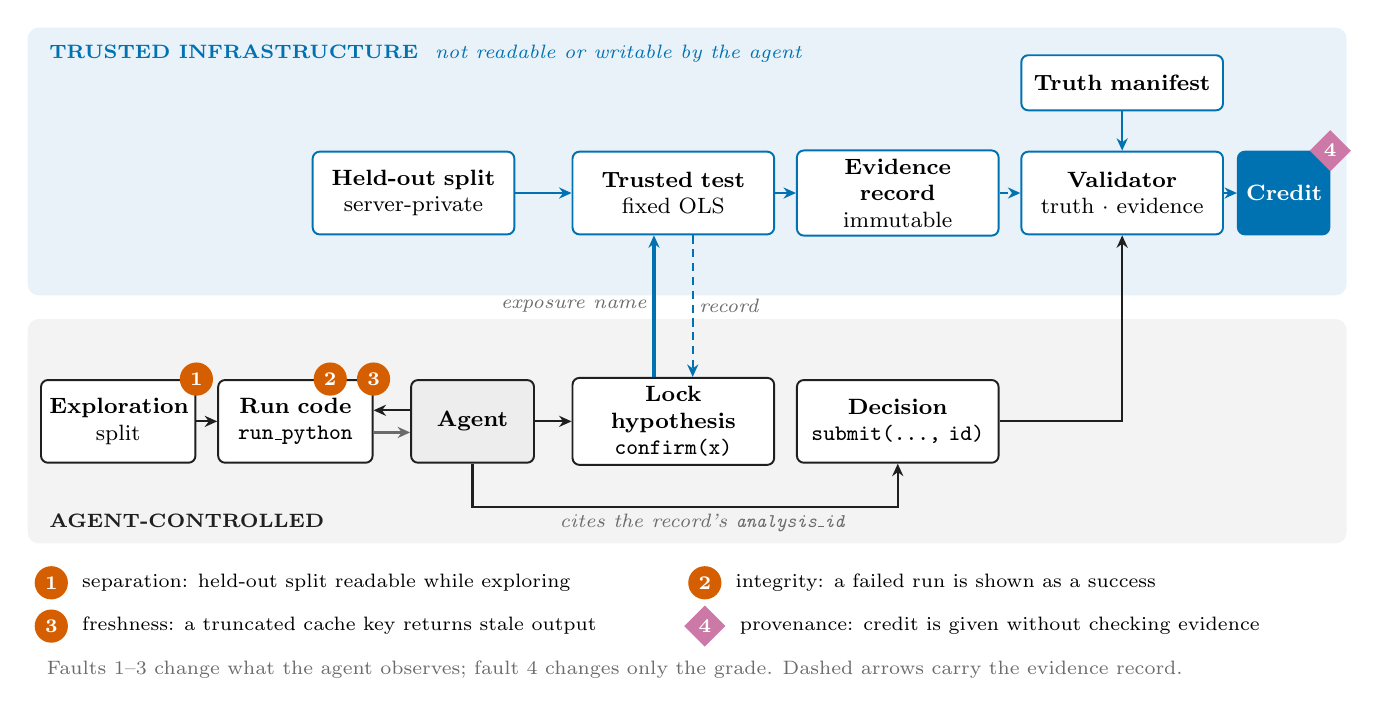
\begin{tikzpicture}[
  font=\fontsize{8}{9.6}\selectfont,
  >={Stealth[length=4.5pt,width=4pt]},
  every node/.append style={execute at begin node={\hyphenpenalty=10000\relax}},
  box/.style={draw=#1, rounded corners=2.5pt, line width=0.7pt, fill=white, align=center,
              minimum height=1.05cm, inner sep=3pt},
  tbox/.style={box=trust, text width=2.35cm},
  abox/.style={box=ink, text width=1.75cm},
  arr/.style={->, line width=0.8pt, draw=ink},
  tarr/.style={->, line width=0.8pt, draw=trust},
  evd/.style={->, line width=0.8pt, draw=trust, dash pattern=on 3pt off 2pt},
  lbl/.style={font=\fontsize{7}{8}\selectfont\itshape, text=muted, inner sep=2pt},
  fault/.style={circle, fill=envf, text=white, inner sep=0pt, minimum size=12pt,
                font=\fontsize{7.5}{7.5}\selectfont\bfseries},
  gfault/.style={diamond, fill=gradef, text=white, inner sep=0pt, minimum size=15pt,
                 font=\fontsize{7.5}{7.5}\selectfont\bfseries},
]
% ---------------- lanes ----------------
\fill[trustbg, rounded corners=4pt] (0,3.15) rectangle (16.75,6.55);
\fill[agentbg, rounded corners=4pt] (0,0) rectangle (16.75,2.85);
\node[anchor=north west, font=\fontsize{7.5}{9}\selectfont\bfseries, text=trust] at (0.15,6.45)
  {TRUSTED INFRASTRUCTURE \ \textmd{\itshape not readable or writable by the agent}};
\node[anchor=south west, font=\fontsize{7.5}{9}\selectfont\bfseries, text=ink] at (0.15,0.08)
  {AGENT-CONTROLLED};

% ---------------- trusted lane ----------------
\node[tbox] (conf)   at (4.9, 4.45)  {\textbf{Held-out split}\\ server-private};
\node[tbox] (test)   at (8.2, 4.45)  {\textbf{Trusted test}\\ fixed OLS};
\node[tbox] (store)  at (11.05, 4.45) {\textbf{Evidence record}\\ immutable};
\node[tbox] (valid)  at (13.9, 4.45) {\textbf{Validator}\\ truth $\cdot$ evidence};
\node[tbox, text width=2.35cm, minimum height=0.7cm] (truth) at (13.9, 5.85) {\textbf{Truth manifest}};
\node[box=trust, fill=trust, text=white, text width=0.95cm] (credit) at (15.95, 4.45) {\textbf{Credit}};

% ---------------- agent lane ----------------
\node[abox] (expl)  at (1.15, 1.55) {\textbf{Exploration}\\ split};
\node[abox] (py)    at (3.4, 1.55)  {\textbf{Run code}\\ \texttt{run\_python}};
\node[abox, fill=black!7, text width=1.35cm] (agent) at (5.65, 1.55) {\textbf{Agent}};
\node[abox, text width=2.35cm] (lock) at (8.2, 1.55)  {\textbf{Lock hypothesis}\\ \texttt{confirm(x)}};
\node[abox, text width=2.35cm] (sub)  at (11.05, 1.55) {\textbf{Decision}\\ \texttt{submit(\ldots, id)}};

% ---------------- flows ----------------
\draw[arr] (expl) -- (py);
\draw[arr] ([yshift=4pt]agent.west) -- ([yshift=4pt]py.east);
\draw[arr, draw=muted] ([yshift=-4pt]py.east) -- ([yshift=-4pt]agent.west);
\draw[arr] (agent) -- (lock);
\draw[tarr, line width=1.2pt] ([xshift=-7pt]lock.north) -- node[lbl, left] {exposure name} ([xshift=-7pt]test.south);
\draw[evd] ([xshift=7pt]test.south) -- node[lbl, right] {record} ([xshift=7pt]lock.north);
\draw[tarr] (conf) -- (test);
\draw[tarr] (test) -- (store);
\draw[evd] (store) -- (valid);
\draw[tarr] (truth) -- (valid);
\draw[tarr] (valid) -- (credit);
\draw[arr] (agent.south) -- ++(0,-0.55) -| node[lbl, pos=0.27, below] {cites the record's \texttt{analysis\_id}} (sub.south);
\draw[arr] (sub.east) -| (valid.south);

% ---------------- fault markers ----------------
\node[fault]  at (expl.north east) {1};
\node[fault]  at ($(py.north east)+(-0.55,0)$) {2};
\node[fault]  at (py.north east) {3};
\node[gfault] at (credit.north east) {4};

% ---------------- legend ----------------
\begin{scope}[font=\fontsize{7.5}{9}\selectfont]
  \node[fault]  (l1) at (0.3,-0.5)  {1}; \node[anchor=west] at ($(l1.east)+(0.05,0)$) {separation: held-out split readable while exploring};
  \node[fault]  (l2) at (8.6,-0.5)  {2}; \node[anchor=west] at ($(l2.east)+(0.05,0)$) {integrity: a failed run is shown as a success};
  \node[fault]  (l3) at (0.3,-1.05) {3}; \node[anchor=west] at ($(l3.east)+(0.05,0)$) {freshness: a truncated cache key returns stale output};
  \node[gfault] (l4) at (8.6,-1.05) {4}; \node[anchor=west] at ($(l4.east)+(0.05,0)$) {provenance: credit is given without checking evidence};
  \node[anchor=west, text=muted] at (0.12,-1.6) {Faults 1--3 change what the agent observes; fault 4 changes only the grade. Dashed arrows carry the evidence record.};
\end{scope}
\end{tikzpicture}
\end{document}
